\chapter{Výsledky studentské práce}




\section{Návrh výsledného systému} \label{sec:Navrh_systemu}

V kapitole je popsán návrh výsledného systému. Skládá se z několika částí: uživatelského rozhraní, algoritmů pro extrakci parametrů z hudební nahrávky, algoritmu generujícího spectoda kód na základě získaných informací a databáze bloků. Podkapitoly podrobně popisují návrh každé části systému.

\subsection{Uživatelské rozhraní} \label{sec:User_interface}

Jedná se o jednoduché webové rozhraní, ve kterém uživatel vloží hudební skladbu ve formátu .wav nebo mp3. Rozhraní obsahuje pole pro vložení nahrávky, které umožňuje výběr ze souborů v uživatelově úložišti. Níže se nachází posuvník se čtyřmi základními hodnotami pro výběr nálady
\texttt{mood}. Jedná se o hodnoty \uv{chill}, \uv{hang out}, \uv{feeling happy} a \uv{dancing}, které jsou v tomto pořadí umístěny na posuvníku viz obrázek \ref{fig:Uzivatelske_rozhrani}. Uživatel může pomocí posouvání posuvníku vybrat pro jakou náladu chce vytvořit animaci. Pod posuvníkem pro výběr nálady se nachází tlačítko spouštějící proces generování Spectoda kódu.
Poslední částí webového rozhraní je textové pole, ve kterém se zobrazí vygenerovaný kód. Na blokovém schématu \ref{fig:User_interaction_diagram} je zobrazen proces postupu uživatele skrze webové rozhraní. 

 \begin{figure}[H]
    \centering
    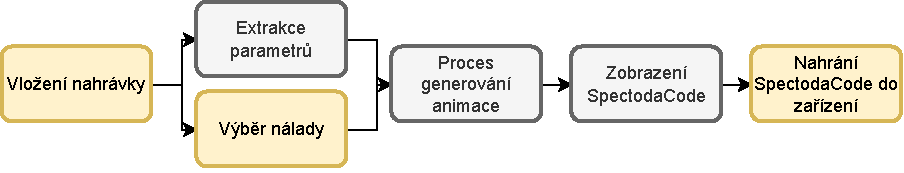
\includegraphics[width = 1\linewidth]{obrazky/User_interaction_diagram.pdf}
    \caption{Blokové schéma postupu uživatele webovou aplikací}
    \label{fig:User_interaction_diagram}
\end{figure}

\subsection{Parametry hudební nahrávky} \label{sec:Parametry_nahravky}
Systém pro generování spectoda kódu popsaný v bodě \ref{sec:System_generovani_animaci} vyžaduje vstupní data o hudební nahrávce. Tato data jsou rozdělena na 7 parametrů. Každý z parametrů představuje vlastnost analyzované nahrávky. Tyto vlastnosti jsou získány pomocí technik popsaných v bodě \ref{sec:Exktrakce_vlastnosti_metody}. Jednotlivé vlastnosti a jejich datové struktury jsou shrnuty v následujících bodech.

\begin{description}
    \item[Detekce dob] -- představuje pole hodnot jehož délka je závislá na době trvání nahrávky. Jednotlivé hodnoty pak udávají časy hudební nahrávky, ve kterých se doby nacházejí. V rámci detekce dob je vypočítána i obálka síly nástupů jednotlivých not. Jedná se o pole hodnot spektrálního toku. 
    
    \item[Tempo skladby] -- je číslo typu float s jednotkou \acs{BPM} vyjadřující počet úderů za minutu. Hodnota BPM se typicky vztahuje k počtu čtvrťových not za minutu \cite{Harvard_dictionary_of_music}. Vybraný algoritmus z knihovny Librosa neumožňuje rozeznat o jaké doby se jedná. Tempo je určeno jako počet detekovaných úderů za minutu. Postup zjištění tempa je popsán v bodě \ref{sec:Librosa}.

    \item[Chroma vektory] -- jsou získány v podobě dvourozměrného pole. Počet řádků pole je dán dvanácti půltóny. Délka pole je závislá na délce nahrávky a velikosti okna při výpočtu \acs{STFT}. V použitých metodách je velikost okna nastavena na 512 vzorků. Z chroma vektorů je spočítána paleta barev dané nahrávky. Paleta barev je uložena jako pole dvanácti hodnot. Pro každý půltón jedna barva. Generování barev je popsáno více v bodech \ref{sec:Color_palete} a \ref{sec:Parameter_extraction}.

    \item[Hlasitost] -- představuje normalizovanou vnímanou úroveň hlasitosti skladby s ohledem na vlastnosti lidského ucha popsané psychoakustikou. Je počítána pro celou skladbu, nebo její část/segment a je značena v jednotkách \acs{LUFS}. Metoda výpočtu hlasitosti je popsána v bodě \ref{sec:Dynamika}.

    \item[Segmentace] -- rozděluje nahranou skladbu do segmentů, ve kterých se objevují stejné hudební tvary. Segmenty jsou uloženy jako pole časů hranic segmentů, kde hranice představuje konec jednoho segmentu a začátek druhého. 

    \item[Žánr] -- je pro zvolenou nahrávku uložen v proměnné \texttt{genre} pomocí slovníku deseti žánrů, ke kterým je přiřazena jejich pravděpodobnost. Protože se v hudbě vyskytuje velké množství žánrů, které se mezi sebou prolínají nejde s přesnou jistotou zařadit každou nahrávku přesně k jednomu žánru. Proto je využito hodnot pravděpodobností. Použité žánry jsou popsány v úryvku kódu \ref{code:song_genre_variables}.
    \begin{figure}[H]
        \begin{lstlisting} [
            caption = {Hodnoty proměnné \texttt{genre}},
            captionpos=b,
            label = {code:song_genre_variables}]
            # Song genre constants
            BLUES       = "blues"
            CLASSICAL   = "classical"
            COUNTRY     = "country"
            DISCO       = "disco"
            HIPHOP      = "hiphop"
            JAZZ        = "jazz"
            METAL       = "metal"
            POP         = "pop"
            REGGAE      = "reggae"
            ROCK        = "rock"
        \end{lstlisting}
    \end{figure}

    \item[Nálada] -- představuje proměnou \texttt{mood} typu float s přednastavenými statickými hodnotami zobrazenými v části kódu \ref{code:song_mood_variables}. Náladu zadává uživatel při nahrávání zvolené skladby.  
    \begin{figure}[H]        
        \begin{lstlisting}[
            caption = {Hodnoty proměnné \texttt{mood}},
            captionpos=b,
            label = {code:song_mood_variables}]
            # Song mood constants
            CHILL       = 0
            HANG_OUT    = 1
            HAPPY       = 2
            DANCING     = 3
        \end{lstlisting}
    \end{figure}
    
\end{description}

\subsection{Databáze bloků animací} \label{sec:Database_structure}
Jak je popsáno v bodě \ref{sec:Spectoda} systém Spectoda obsahuje základní animace, které jsou skládány do bloků a tím vznikají komplexní struktury. Systém využívá již připravených bloků animací, které jsou uloženy jako objekty. Těmto objektům jsou přiřazeny parametry \texttt{code}, \texttt{characteristics}, \texttt{length} a \texttt{colors}. Jejich struktura je zapsaná datovou třídou \texttt{AnimationBlock}. Z těchto objektů třídy jsou dále tvořeny datasety zapsané třídou \texttt{Dataset}. Tyto instance obsahují pět bloků animací a parametry \texttt{genre}, \texttt{tempo} a \texttt{mood}. UML diagramy tříd jsou zobrazeny na obrázku \ref{fig:UML_diagram_Dataset_AnimationBlock}.

\begin{figure}[H]
    \centering
    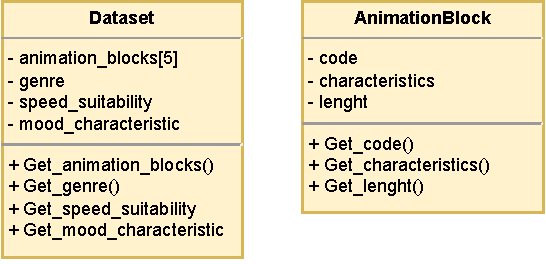
\includegraphics[width = 0.7\linewidth]{obrazky/UML_diagram_Dataset_and_AnimationBlock.pdf}
    \caption{Blokové diagramy tříd \texttt{Dataset} a \texttt{AnimationBlock}}
    \label{fig:UML_diagram_Dataset_AnimationBlock}
\end{figure}

Jak bylo zmíněno bloky animací mají proměnou \texttt{characteristic}, která je rozděluje do pěti kategorií. Každá kategorie má svůj specifický význam: 

\begin{itemize}
    \item BANG -- Vhodné pro začátek krátkých segmentů. Velmi úderné a rychlé.
    \item SHOT -- Rychlé animace pro kratší segmenty.
    \item PULL -- Úderné animace, které vtáhnou do děje na začátku delších segmentů.
    \item THEME -- Primární animace pro delší segmenty obsahuje hlavní téma.
    \item FLOW -- Dlouhé pomalé animace pro vyplnění klidných částí skladby.
\end{itemize}

\begin{figure}[H]
    \begin{lstlisting}[
        caption = {Hodnoty proměnné \texttt{characteristics}},
        captionpos=b,
        label = {code:anim_characteristic_constants}]
        # Animation characteristics constants
        BANG        = 0
        SHOT        = 1
        PULL        = 2
        THEME       = 3
        FLOW        = 4
    \end{lstlisting}
\end{figure}

\subsection{Systém pro generování animací} \label{sec:System_generovani_animaci}
Systém pro generování animací je jádrem práce. Jeho struktura udává vizuální kvalitu animací a schopnost přizpůsobit se různorodým skladbám. V této kapitole je popsána jeho vnitřní logika.

První částí systému je vstupní rozhraní, ve kterém jsou přijímány data obsahující vlastnosti hudební nahrávky. Struktura přijímaných dat je popsána v bodě \ref{sec:Parametry_nahravky}. Každý ze zmíněných parametrů plní důležitou funkci v rozhodovacím procesu skládání bloků animace. Níže jsou popsány rozhodovací funkce pro jednotlivé parametry.

\begin{description}
    \item[Žánr a nálada] -- jsou používány pro výběr vhodného balíčku animací. Tyto balíčky jsou nazývány datasety a jejich datová struktura je popsána v bodě \ref{sec:Database_structure}. Postup výběru datasetu je následující. Každý dataset obsahuje konstantní hodnotu nálady \texttt{mood} a seznam všech deseti používaných žánrů. Ke každému žánru je přiřazeno racionální číslo udávající hodnotu jak moc je dataset pro daný žánr vhodný. Kde 1 je nejvíce vhodný a 0 nejméně. Na základě seznamu \texttt{genre} dochází k postupnému seřazení všech, datasetů dle jejich vhodnosti pro nahraný audio soubor a výběru pěti nejvíce se hodících. V dalším kroku jsou vyřazeny všechny datasety, které neodpovídají zvolené náladě \texttt{mood}. Programové řešení výběru vhodného datasetu je popsáno v bodě \ref{sec:Vyber_datasetu}.
    
    \begin{figure}[H]
        \centering
        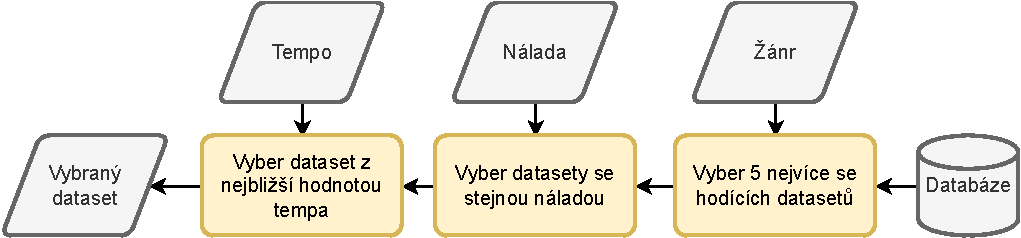
\includegraphics[width = 1\linewidth]{obrazky/Dataset_selection_diagram.pdf}
        \caption{Blokový diagram výběru datasetu.}
        \label{fig:Dataset_selection_diagram}
    \end{figure}

    \item[Tempo skladby] -- je poslední hodnotou při výběru vhodného datasetu.    Všechny zbývající datasety jsou porovnány s odhadovaným tempem skladby a je stanoven rozdíl jejich hodnot. Jako výsledný dataset je vybrán ten, který má hodnotu rozdílu tempa nejmenší. Celý postup je znázorněn na obrázku \ref{fig:Dataset_selection_diagram}.
    
    \item[Segmentace] -- má důležitou roli při výběru vhodných bloků animací. U každého ze segmentů je počítána jeho délka a hlasitost. Tyto údaje jsou pak porovnávány vůči celé skladbě. Na základě těchto údajů jsou segmenty děleny na: hlasité, tiché, krátké a dlouhé. Práce se segmenty v programu je popsána v bodě \ref{sec:Vyber_bloku_animace}

    \item[Detekce dob] -- udává časy, kde se v nahrávce nacházejí doby. V aplikaci je tento parametr důležitý zejména pro správné umístění začátku a konce animace tak, aby seděla do rytmu. 

    \item[Obálka síly nástupů] -- z anglického pojmu onset strength envelope, je hodnota na základě které je určena významnost jednotlivých dob. Tato významnost je brána jako nejvyšší hodnota obálky síly nástupů v okolí dané doby.
     
    \item[Chroma vektory] -- udávají tónovou strukturu skladby v průběhu času. Tento parametr je využit pro nastavení barev animace. Chroma vektory se analyzují a jsou vybrány 3 hlavní tóny nejčastěji znějící v nahrávce. Každému z tónů je přiřazen barevný odstín tak, aby se jednalo o barvy triadické. Zbývajícím tónům jsou přiřazeny odstíny těchto barev a jsou uloženy jako barevná paleta nahrávky. U jednotlivých animací jsou na základě počtu barev v údaji \texttt{colors} z chroma vektorů vypočítány nejvíce se vyskytující tóny. Na základě těchto tónů jsou animaci přiřazeny barvy z palety barev. Celý proces generování a přiřazování barev je popsán v bodě \ref{sec:Color_palete}.

    \item[Hlasitost] -- pomáhá při procesu segmentace. Refrén a sloka se mohou lišit hlasitostí. Hlasitost je počítána pro celou skladbu a následně pro segmenty. Při výběru vhodného bloku animace dochází k porovnání hlasitosti segmentu vůči hlasitosti nahrávky. Na základě porovnání je určeno jak výrazné mají být animace v daném segmentu. Vyšší hodnoty představují rychlejší a údernější animace. Nižší hodnoty naopak pomalejší a klidnější animace.
\end{description}


Druhá část systému tvoří samotnou logiku skládání bloků animací. Rozhodovací struktura lze zjednodušit na několik po sobě jdoucích kroků znázorněných blokovým diagramem na obrázku \ref{fig:diagram_procesu_generovani_animaci}. V bodech níže jsou postupně popsány všechny kroky.

\begin{figure}[H]
    \centering
    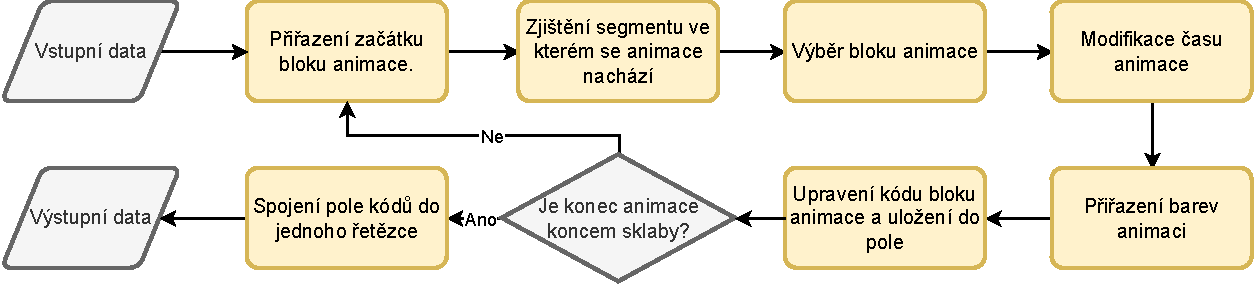
\includegraphics[width = 1\linewidth]{obrazky/UML_diagramy_anim_generation_process.pdf}
    \caption{Blokový diagram procesu generování animací}
    \label{fig:diagram_procesu_generovani_animaci}
\end{figure}

\begin{itemize}
    \item  
    Prvním z bloků je přiřazení času začátku animace. Pokud se jedná o počáteční animaci ve skladbě, je čas začátku automaticky přiřazen jako čas, ve kterém se nachází první doba. Pro každou další animaci je volen čas začátku jako konec animace předchozí.
    \item 
    Druhým krokem je nalezení segmentu, ve kterém se začátek animace nachází. Segment je vyjádřen jako jeho hranice začátku a konce. Tyto hranice jsou nalezeny v poli hranic segmentů jako nejbližší nižší a nejbližší vyšší hodnota času k času začátku animace. Funkce pro vyhledání segmentu je zobrazena v úryvku kódu \ref{code:Find_segment}. 

    \item 
    Třetím krokem v pořadí je výběr vhodného bloku animace. Výběr vhodného bloku je důležitý pro výsledný pocit z konečné animace. Ze získaných parametrů o nahrávce je vypočítáno dalších 7 hodnot. Na získané hodnoty jsou aplikovány váhy a poté jsou mezi sebou porovnány. Výsledkem procesu jsou 3 proměnné typu boolean představující otázky: Je segment dlouhý? Je segment hlasitý? Je doba začátku animace důležitá v segmentu? Je doba začátku animace důležitá v nahrávce? Pro lepší představu je struktura procesu zobrazená na blokovém diagramu \ref{fig:Anim_block_param_selection_diagram}. Na základě získaných logických proměnných je pomocí rozhodovací struktury vybrána vhodná charakteristika animace. Struktura je tvořena dvěma kroky a v každém kroku jsou 4 řešení. Výsledný počet řešení je tedy $2^4 = 16$. Nejprve je porovnáváno jestli je segment dlouhý a hlasitý. Kombinace těchto dvou stavů (ano/ne) tvoří první čtyři zmíněné řešení. Ve druhém kroku je porovnávána důležitost počáteční doby animace v segmentu a skladbě. Toto porovnání nabývá také 4 možných řešení.  

    \begin{figure}[H]
        \centering
        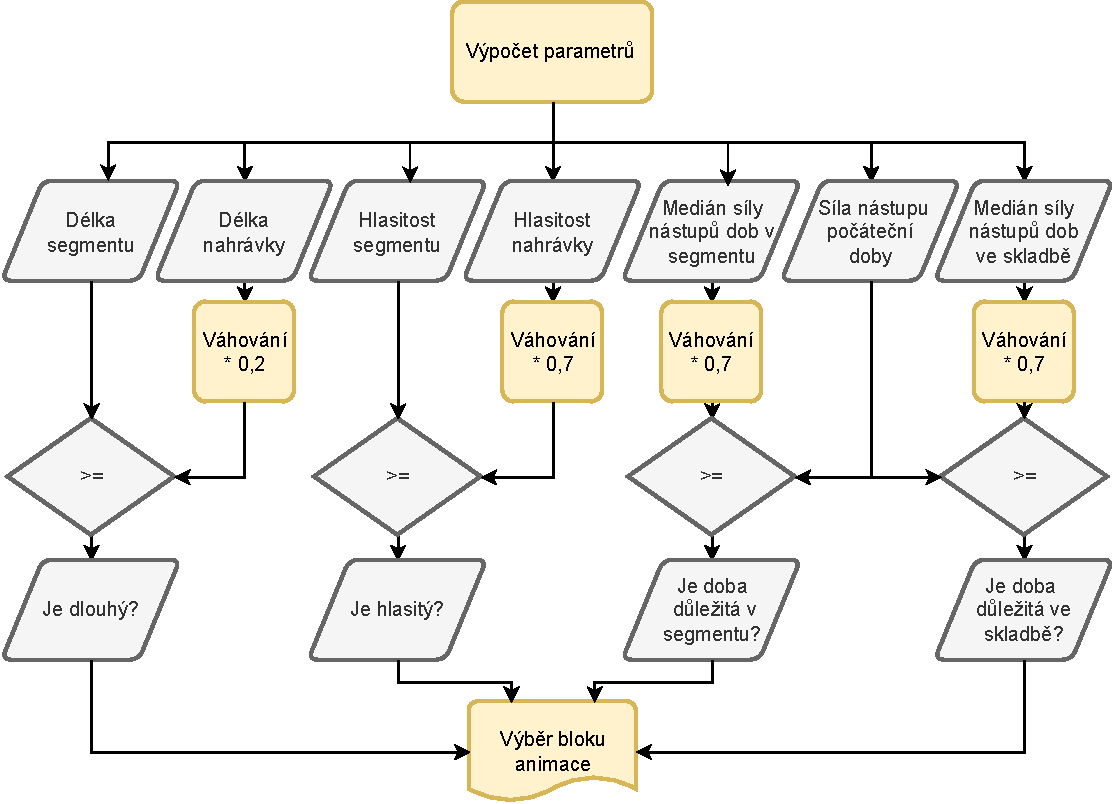
\includegraphics[width = 1\linewidth]{obrazky/UML_diagramy_anim_bock_selection _part_1.pdf}
        \caption{Blokový diagram procesu výpočtu parametrů pro výběr animace}
        \label{fig:Anim_block_param_selection_diagram}
    \end{figure}

    \item Poté co je vybrán vhodný blok animace je důležité upravit její délku tak, aby končila opět na době. Každý blok má nastavenou doporučenou délku uloženou v proměnné \texttt{anim\_length}. Nejprve je vypočítán čas konce animace jako součet začátku animace a její doporučené délky. Pomocí funkce \texttt{Find\_nearest\_beat} zobrazené v úryvku kódu \ref{code:Find_nearest_beat} je nalezena doba, která má nejmenší časový rozdíl od vypočítaného konce animace. Nyní je známa doba na které bude animace konči, ještě je ale potřeba vypočítat modifikátor, který upraví délku animace tak, aby na ní skutečně skončila. Modifikátor je číslo, kterým je násobena doporučená délka animace tak aby odpovídala délce mezi vybranou počáteční dobou a koncovou dobou. Výpočet je znázorněn rovnicemi \ref{rov:time_modifier}, kde $M$ je modifikátor, $T_a$ je doporučený čas animace, $T_n$ je nový čas animace, $T_{eb}$ je čas ve kterém se nachází konečná doba animace a $T_{sb}$ je čas ve kterém se nachází počáteční doba animace.
    
    \begin{equation}
        M = \frac{T_a}{T_n} = \frac{T_a}{T_{eb} - T_{sb}}
        \label{rov:time_modifier}
    \end{equation}
    
    \item Nyní je možné vybrat barvy z palety barev dané nahrávky. Nejprve jsou z chroma vektorů vypočítány tóny, které zní nejdéle v časovém rozmezí bloku animace. Z proměnné \texttt{anim\_color} uložené v bloku animace zjistíme kolik je potřeba barev. Na základě zjištěného počtu je z palety barev vybráno \textit{n} barev, které odpovídají nejvíce znělým tónům v dané části skladby. 

    \item Šestým krokem je vygenerování kódu animace. Zdrojový kód je uložen v proměnné \texttt{anim\_code} vybraného bloku. Do něj je potřeba na předpřipravená místa vložit získané informace o začátku, konci, rychlosti a barvě. Po vložení těchto informací je v textovém řetězci uložen do pole jako další hotová animace. 
    
    \item Posledním bodem cyklu je kontrola jestli je konec animace poslední dobou ve skladbě. Pokud není cyklus se opakuje stále dokola než je vygenerován kód pro všechny části nahrávky. Po dokončení tohoto procesu je pole vygenerovaných zdrojových kódů sečteno do jednoho dlouhého řetězce jako finální kód animace a je připraven k nahrání do Spectoda zařízení. 
    
\end{itemize}

\section{Metody extrakce parametrů z hudební nahrávky} \label{sec:Exktrakce_vlastnosti_metody}
Díky vědecké komunitě vznikly volně dostupné knihovny obsahující techniky z oborů \acs{MIR}. V této části práce jsou prozkoumány 3 knihovny zmíněné v bodě \ref{sec:Dostupna_reseni}. Jsou porovnány jejich funkce pro získání parametrů z hudební nahrávky. Tyto funkce jsou mezi sebou porovnány z hlediska přesnosti výsledků, rychlosti výpočtů, jednoduchosti použití a možnosti využití pro komerční účely. 

% TODO Když zbude čas, kapitola o licencích a jejich významech (plusy mínusy).

\subsection{Detekce dob a tempa}
Pro porovnání detekce dob jsou vybrány 3 funkce. Pro každou knihovnu jedna funkce. První je z knihovny Librosa funkce \texttt{beat\_track}. Z knihovny Madmom je použit \texttt{BeatTrackingProcessor} a z knihovny Aubio funkce \texttt{tempo}. Funkce jsou porovnány na třech skladbách skupiny Beatles. Níže v grafu \ref{fig:Oh-Darling_beat_analysis} je vidět úryvek skladby Oh-Darling!. Pro lepší zobrazení jsou osy grafu v rozsahu 55 - 65 sekund nahrávky. Na prvním z grafů je vyobrazen mel spektrogram vypočítán pomocí funkce \texttt{mel spectrogram} z knihovny Librosa. Grafy b), c) a d) zobrazují v pozadí obálku síly nástupů a vertikální pruhované čáry znázorňují detekované doby dané funkce. Vertikální modré tečkované čáry jsou referenční doby zaznamenané institucí Centre for digital music na univerzitě Queen Mary, University of London \cite{Isophonic}. 

\begin{figure}[H]
    \centering
    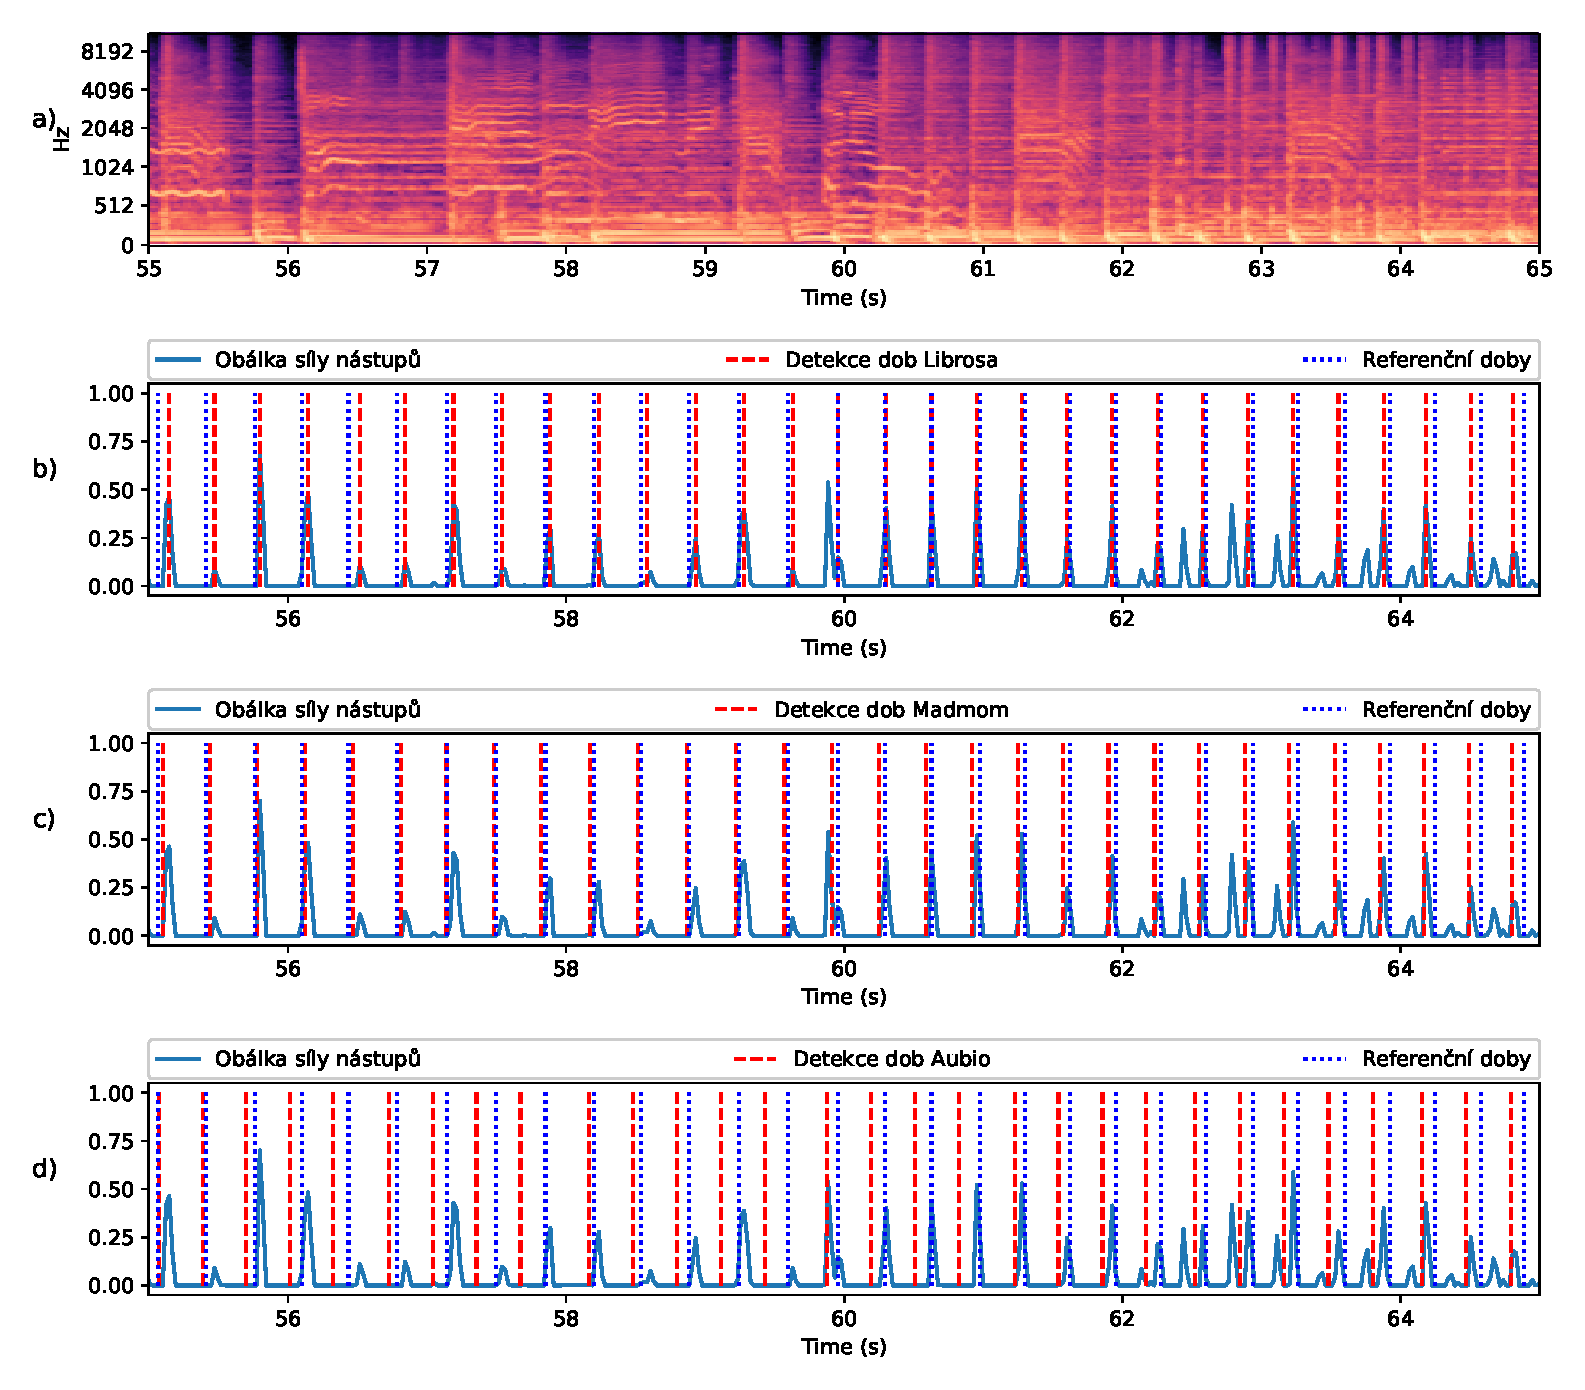
\includegraphics[width = 1\linewidth]{obrazky/Oh-Darling_Beat_analysis_graphs.eps}
    \caption{Porovnání metod detekce dob na úryvku skladby Oh-Darling!. \textbf{a)} Mel spektrogram \textbf{b)}Detekce dob pomocí Librosa \textbf{c)} Detekce dob pomocí Madmom \textbf{d)} Detekce dob pomocí Aubio}
    \label{fig:Oh-Darling_beat_analysis}
\end{figure}

Z grafu lze vidět, že funkce z knihoven Librosa a Madmom se nejvíce přibližují referenčním dobám. Pro přesné hodnocení funkcí je využita knihovna Mir\_eval poskytující funkce pro hodnocení přesnosti detekce dob. Pomocí teto knihovny je počítáno Cemgil skóre. Popis knihovny a výpočtu je zmíněn v bodě \ref{sec:Mir_eval}. Posledním hodnoceným parametrem je doba výpočtu. Výsledky Cemgil skóre, a doby výpočtu pro jednotlivé skladby jsou zobrazeny na obrázku \ref{fig:Beat_tracking_time_and_cemgil}.

\begin{figure}[H]
    \centering
    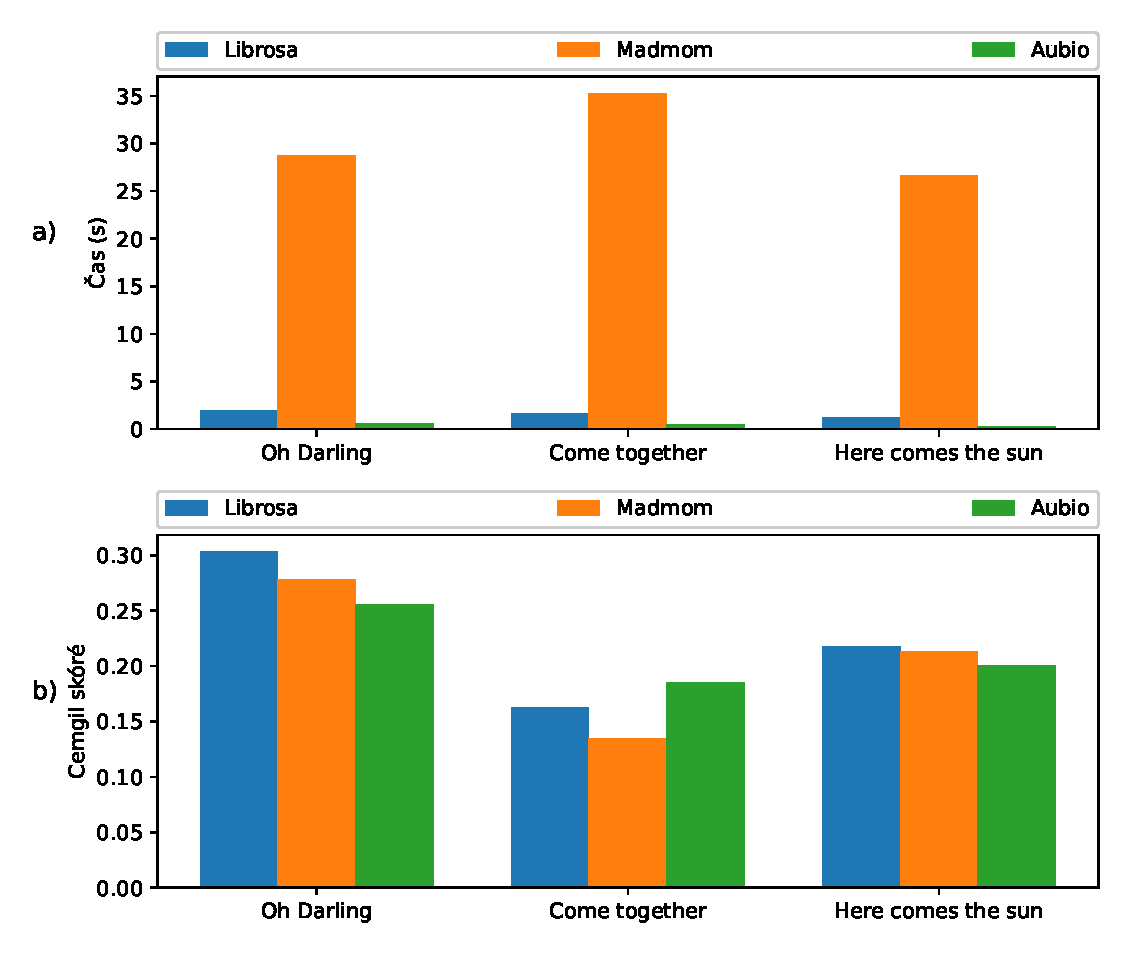
\includegraphics[width = 1\linewidth]{obrazky/Beat_tracking_time_and_cemgil_graphs.eps}
    \caption{Porovnání přesnosti a času metod detekce dob na skladbách Oh-Darling!, Come Together a Here Comes The Sun. \textbf{a)} Čas výpočtu \textbf{b)} Cemgil skóre}
    \label{fig:Beat_tracking_time_and_cemgil}
\end{figure}

Pro systém byla vybrána funkce z knihovny Librosa z důvodů jeho velké přesnosti a rychlosti výpočtů.

\subsection{Analýza chroma vektorů}

Hodnocení vhodné funkce pro výpočet chroma vektorů je realizováno zejména vizuálně na zobrazených grafech referenčních skladeb. Tyto grafy lze vidět na obrázku \ref{fig:Chroma_analysis}. Porovnávány jsou 4 funkce z knihovny librosa \texttt{chroma\_stft}, \texttt{chroma\_cqt}, \texttt{chroma\_cens} a čtvrtou je funkce \texttt{chroma\_cqt} s řetězci předzpracování signálu a filtrací výsledných chroma vektorů. Principy výpočtů jednotlivých funkcí jsou popsány v bodě \ref{sec:Librosa}. Z knihovny Madmom je použit \textit{DeepChromaProcessor}.

\begin{figure}[H]
    \centering
    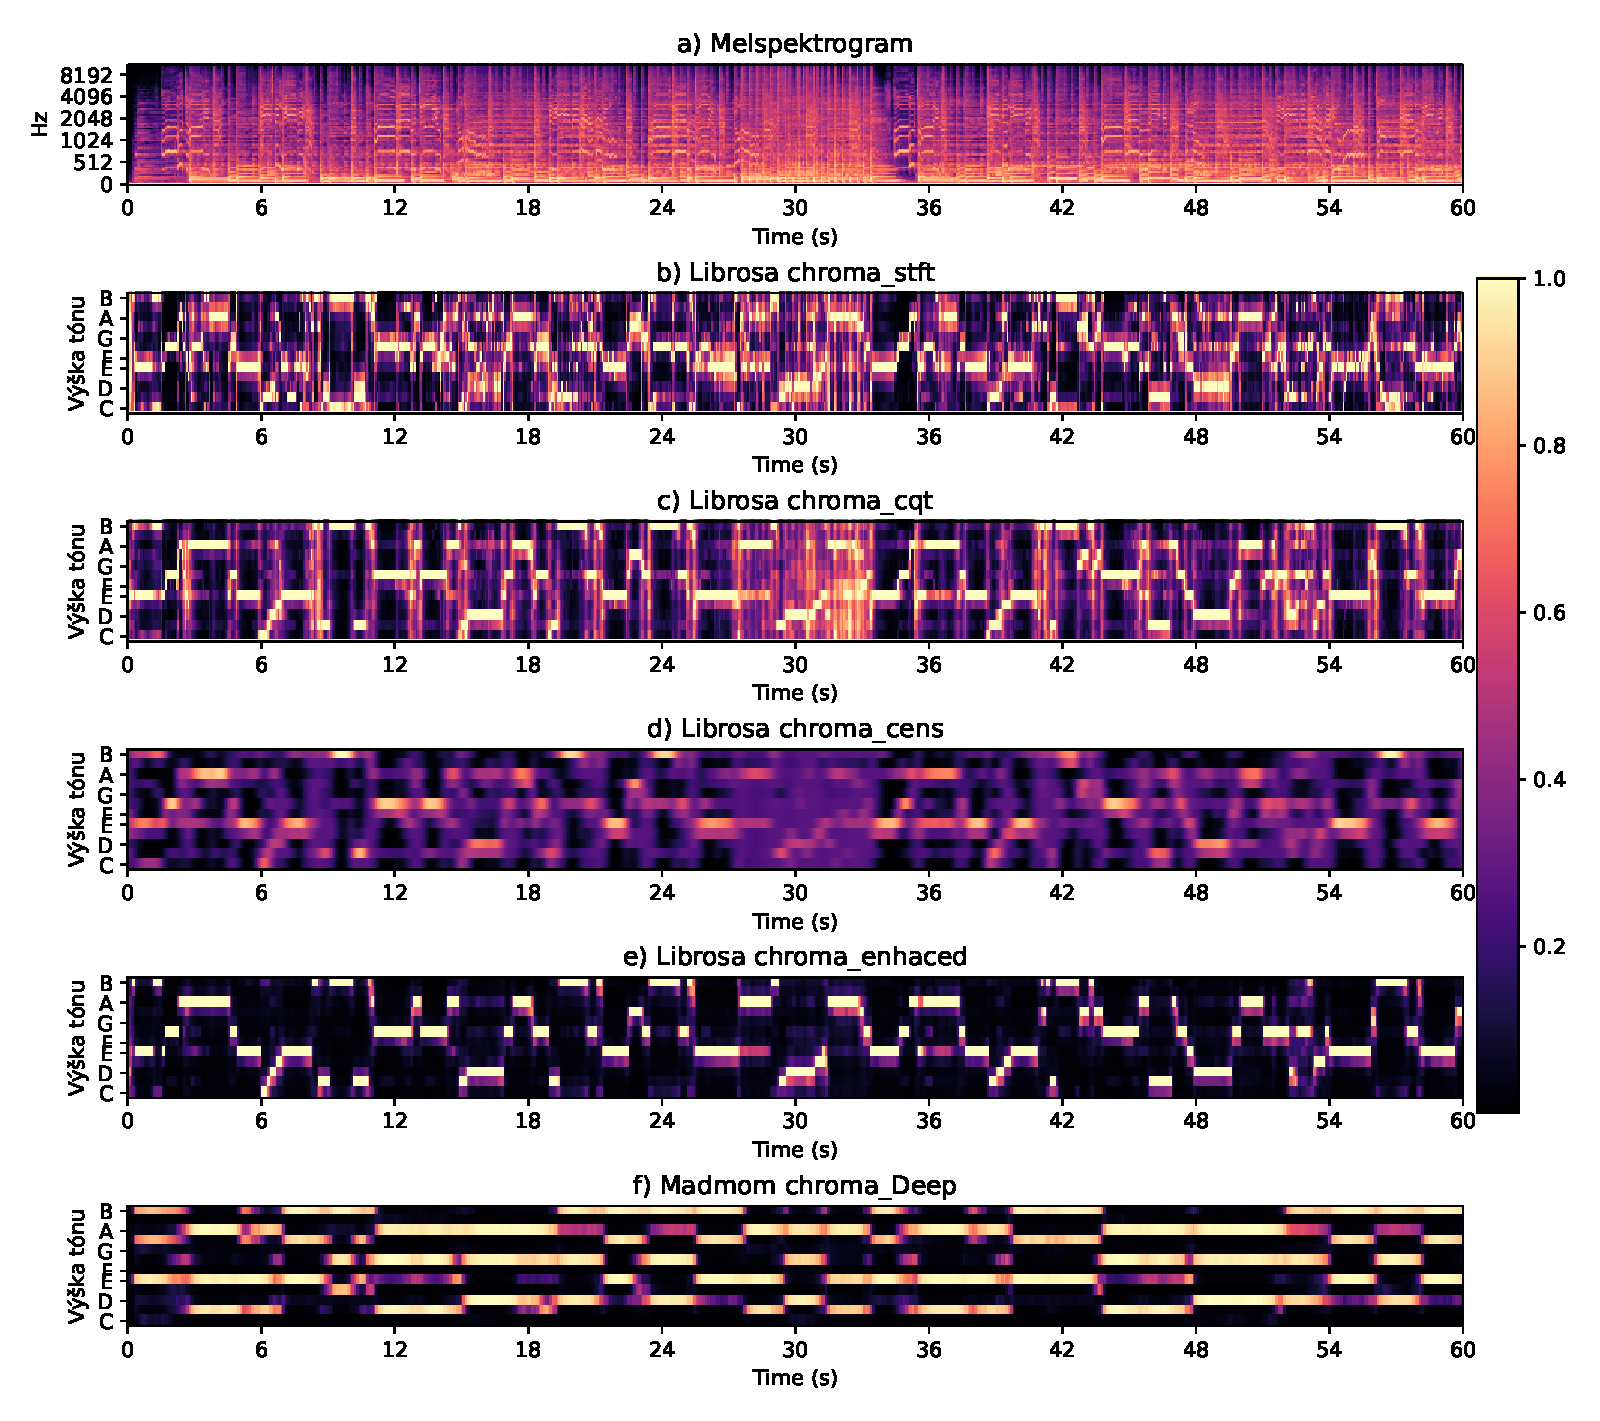
\includegraphics[width = 1\linewidth]{obrazky/Oh-Darling_chroma_analysis_graphs.eps}
    \caption{Porovnání výpočtu chroma vektorů na skladbě Oh-Darling! zkrácená na délku jedné minuty.}
    \label{fig:Chroma_analysis}
\end{figure}

Z obrázku \ref{fig:Chroma_analysis} lze vidět patrný rozdíl v přístupu výpočtu chroma vektorů. U grafů \textit{b)}, \textit{c)} a \textit{d)} lze vidět velké množství šumu. U grafu \textit{e)} je šum vyfiltrován přidanými metodami. Na grafu \textit{f)} lze vidět, že knihovna Madmom a z ní použitý \texttt{DeepChromaProcessor} přistupuje k výpočtu chroma vektorů odlišně. Je využito delší časové okno pro transformaci do frekvenční oblasti. Z toho je patrné, že v časovém měřítku údaj není natolik přesný jako u knihovny Librosa. Pro následné použití v algoritmu pro generování animací je však tento výsledek mnohem stálejší. 

Dalším hodnoceným parametrem je délka výpočtu chroma vektorů. Ta je závislá na složitosti algoritmů jež funkce využívají k výpočtu. Porovnání je zobrazeno na obrázku \ref{fig:Chroma_calculation_time}. Z obrázku je zřejmé, že pomocné metody pro předzpracování a filtraci chroma vektorů z funkce \textit{chroma\_cqt} přidaly značné množství výpočetního času oproti samotnému výpočtu chroma vektorů.

\begin{figure}[H]
    \centering
    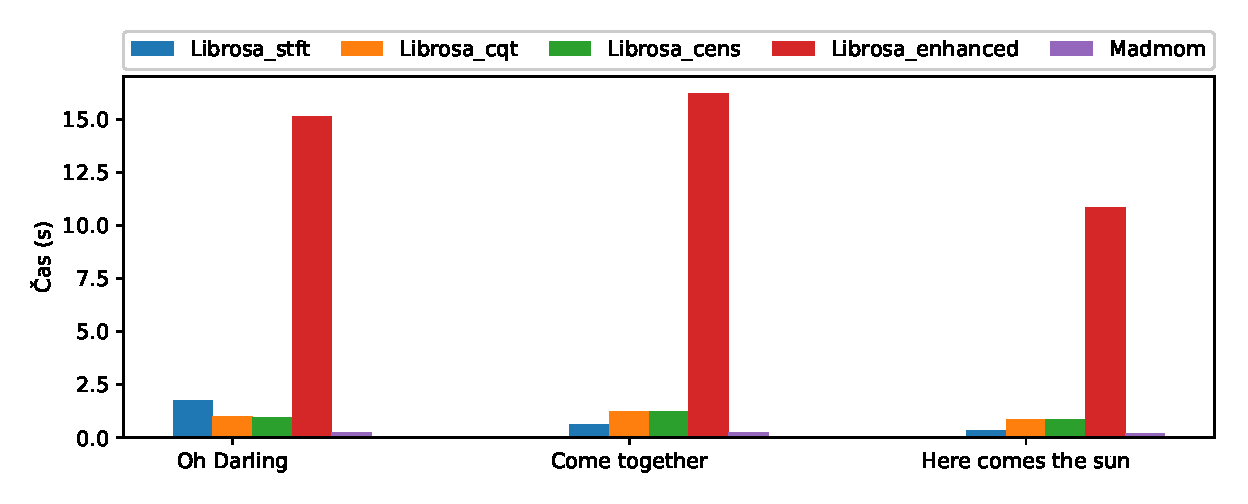
\includegraphics[width = 1\linewidth]{obrazky/Chroma_analysis_times_comparison.eps}
    \caption{Porovnání délky výpočtu chroma vektorů}
    \label{fig:Chroma_calculation_time}
\end{figure}
    
\subsection{Efektivní hodnota signálu}
Výpočet efektivní hodnoty signálu je realizován pomocí funkce z knihovy Librosa. Pro výpočet je použito okno o délce 2048 vzorků. Hodnoty jsou vycentrovány na střed rozsahu okna tedy 1024 vzorků. Získaná křivka je uhlazena pomocí výpočtu klouzavého průměru. Počet vzorků ze kterých se klouzavý průměr vypočítá odpovídá délce signálu $7,5 s$ a je závislý na jeho vzorkovací frekvenci. Získané křivky jsou zobrazeny na obrázku \ref{fig:RMS_calculation}.

\begin{figure}[H]
    \centering
    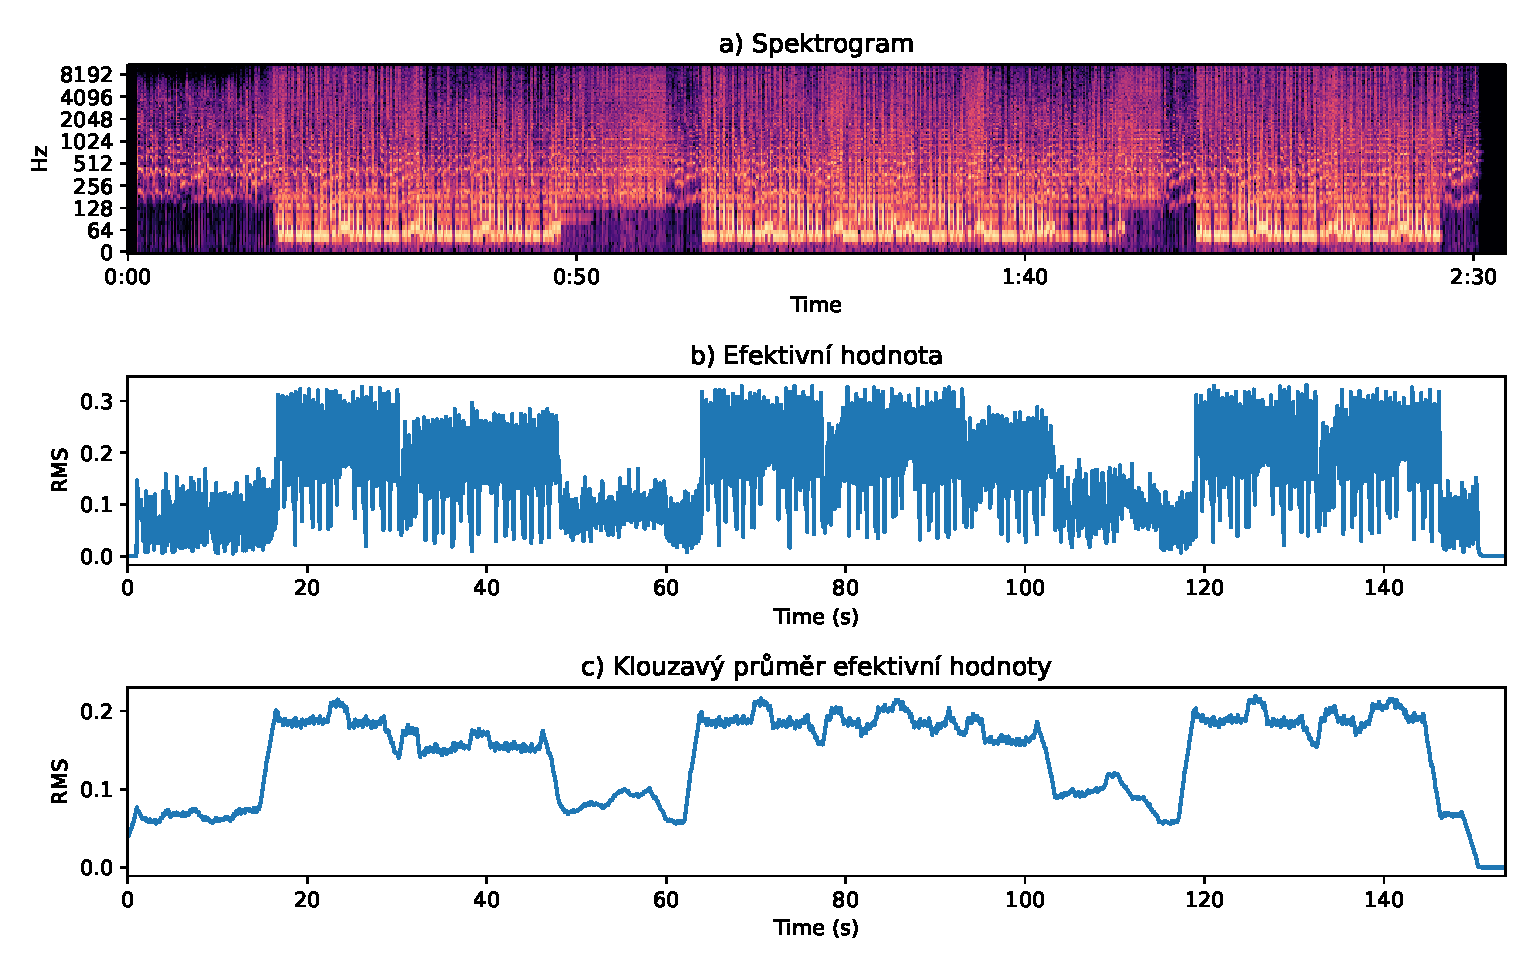
\includegraphics[width = 1\linewidth]{obrazky/Belly_dancer_RMS.eps}
    \caption{Zobrazení efektivní hodnoty skladby Belly dancer}
    \label{fig:RMS_calculation}
\end{figure}

\subsection{Hlasitost} \label{sec:Pyloudnorm}
Pro výpočet hlasitosti skladby nebo jejich částí je použita knihovna \texttt{Pyloudnorm} \cite{Pyloudnorm}. Tato knihovna implementuje standardizovaný algoritmus ITU-R BS.1770 \cite{BS.1770}. Který je více popsaný v bodě \ref{sec:Dynamika}. Výstupní hodnotou funke je číselná hodnota udávající hlasitost skladby nebo jejich částí v jednotkách LUFS. 

\subsection{Segmentace} \label{sec:Segmentace}
Z vybraných knihoven nabízí metody pro segmentaci nahrávky pouze knihovna librosa ve funkci \texttt{agglomerative}. Pro rozdělení na segmenty využívá jako vstupní data chroma vektory. Díky tomu je možné dosáhnou odlišných výsledků použitím různých metod pro výpočet vstupních chroma vektorů. Na obrázku \ref{fig:Segmentation_chroma_comparison} je zobrazeno využití dvou různých přístupů na vliv výpočtu dvanácti segmentů. Prvním z přístupů je porovnání chromagramů získaných zvolenými metodami z knihovny librosa a madmom. Druhým přístupem je jejich přepočet na binární variantu s váhou  $0,6$ kde hodnoty vzorků chroma vektorů nižší nebo rovny jsou zapsány jako 0 a hodnoty vyšší jako 1. Tento proces je využit i při generování palety barev \ref{sec:Color_palete}. Z obrázku je patrné, že největší rozdíl ve stanovení segmentů hraje právě zvolená metoda pro výpočet chroma vektorů. U binární verze pak lze vidět malé odchylky v rámci dvou až tří segmentů. 

\begin{figure}[H]
    \centering
    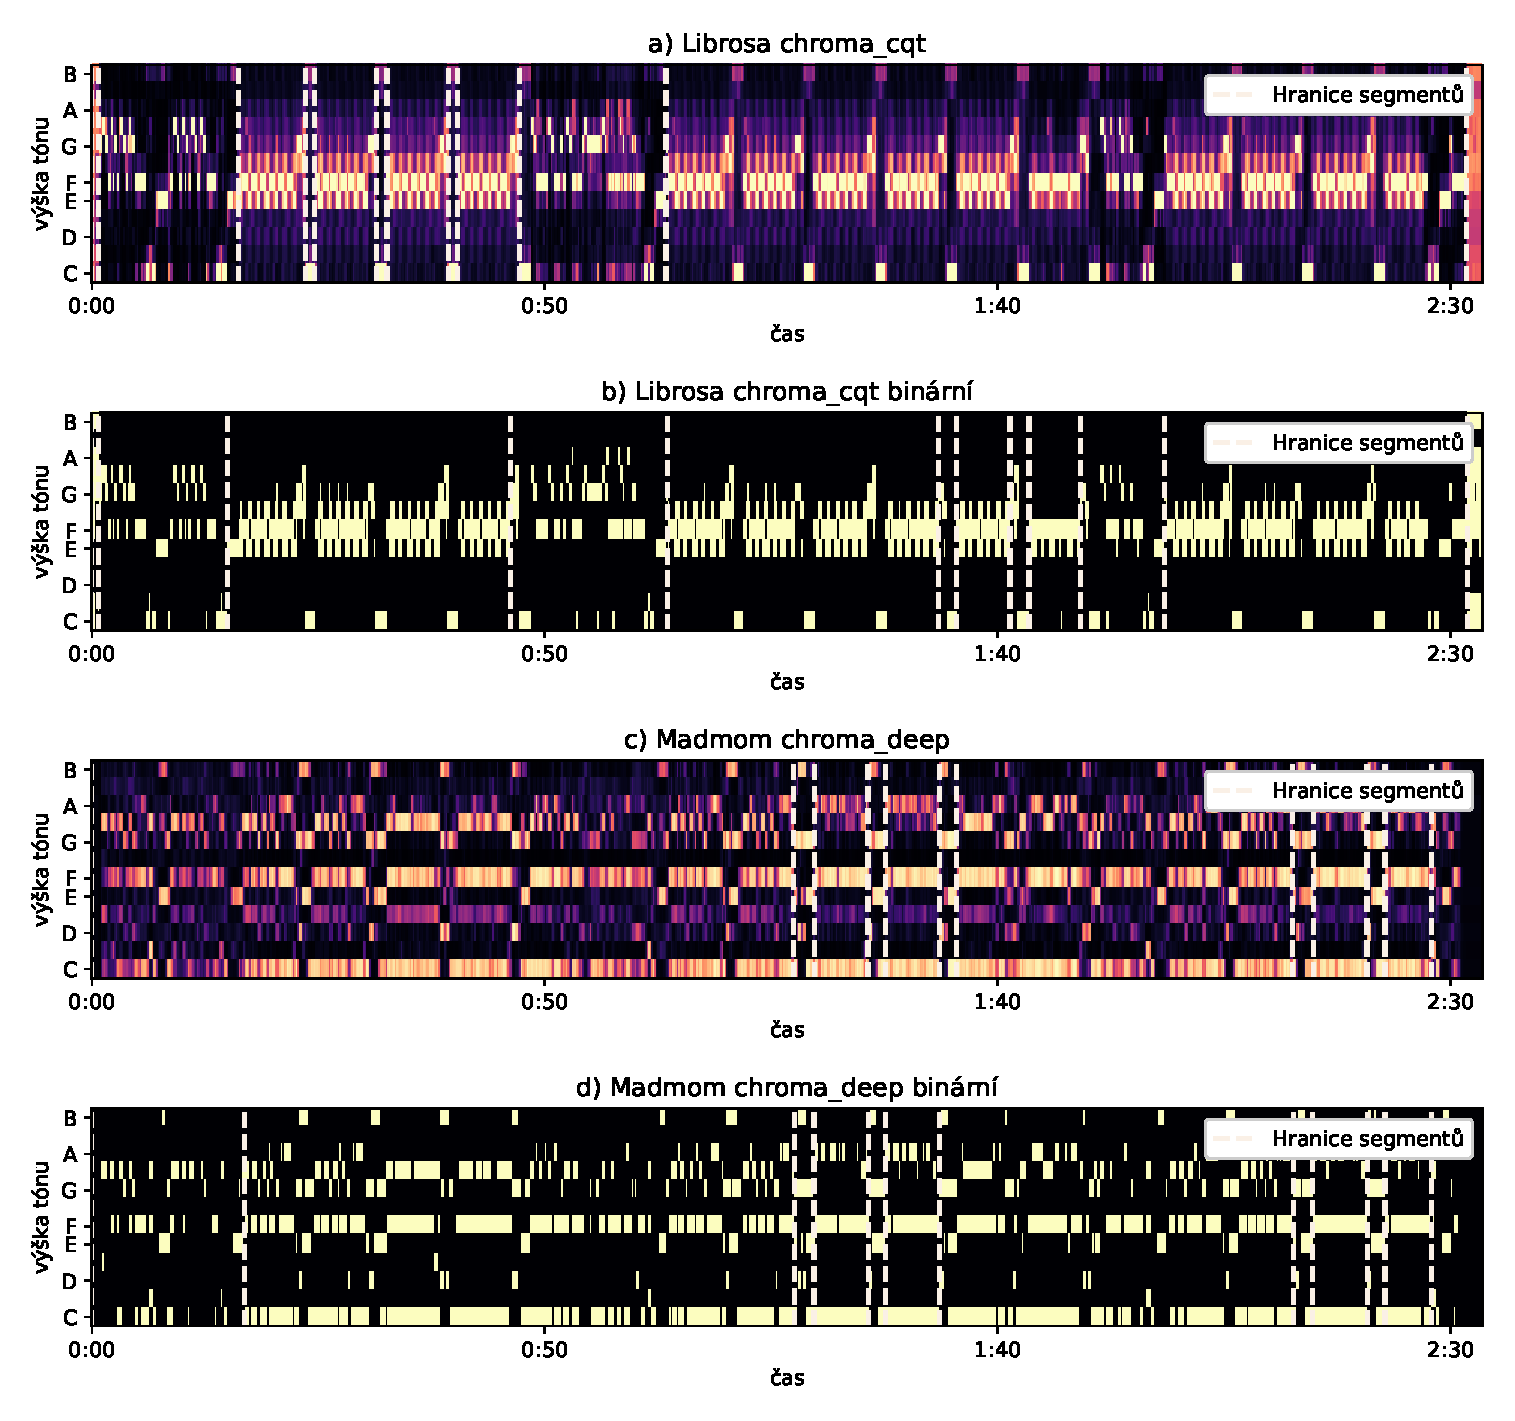
\includegraphics[width = 1\linewidth]{obrazky/Segmentation_chroma_comparisons.eps}
    \caption{Porovnání vlivu výpočtu chroma vektorů na výslednou segmentaci pro 12 segmentů.}
    \label{fig:Segmentation_chroma_comparison}
\end{figure}

\section{Realizace} \label{sec:Realizace}

Kapitola popisuje jakým způsobem bylo dosaženo funkčního prototypu systému pro generování animací na základě parametrů hudební nahrávky. Jsou zde popsány použité programovací jazyky, metody a algoritmy. Podrobně je popsáno programové řešení jednotlivých částí systému. 

\subsection{Uživatelské rozhraní}

Uživatelské rozhraní je reprezentováno webovou stránkou a je naprogramováno pomocí značkovacího jazyka \acs{HTML}\footnote{HTML -- Hypertext markup language. Je značkovací jazyk používaný pro tvorbu webových stránek.} spolu s formátováním v jazyce \acs{CSS}\footnote{CSS -- Cascading style sheets. Je jazyk popisující styl zobrazení HTML elementů\cite{CSS}.}. Aby bylo možné k webové stránce přistupovat veřejně, je nasazena na serveru služby PythonAnywhere. Která poskytuje serverové řešení pro realizaci python aplikací. Funkčnost a propojení webového rozhraní s python systémem pracujícím na pozadí je řešeno pomocí frameworku Flask, který umožňuje jednoduchou interakci webové stránky s python aplikací běžící na pozadí pomocí protokolu HTTP\footnote{HTTP -- Hypertext transfer protocol. Je protokol navržen pro komunikaci mezi klientem a serverem.}. V rámci webové aplikace je využito pouze metod \texttt{GET} a \texttt{POST}. Kde metoda \texttt{POST} slouží pro odeslání dat s přiřazenou nahrávkou a vybranou náladou.

\begin{figure}[H]
    \centering
    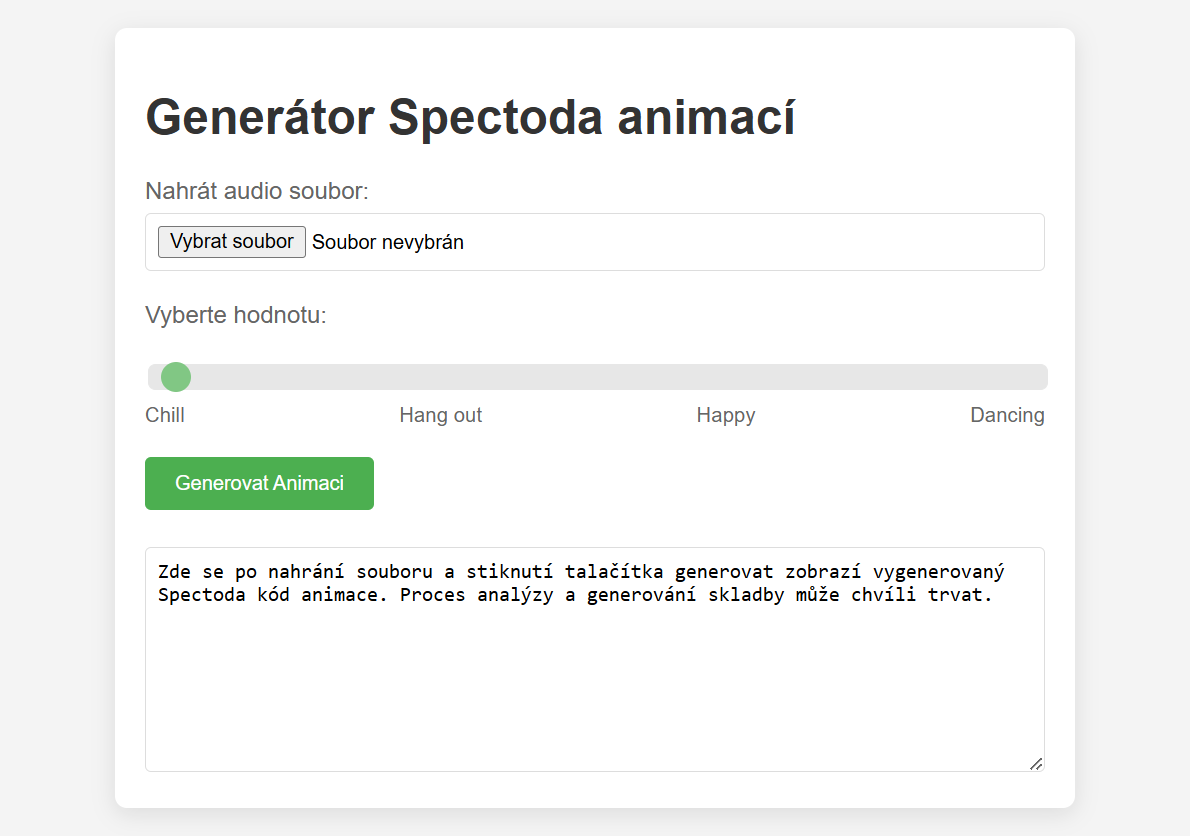
\includegraphics[width = 1\linewidth]{obrazky/Uzivatelske_rozhrani.png}
    \caption{Uživatelské rozhraní aplikace}
    \label{fig:Uzivatelske_rozhrani}
\end{figure}

\subsection{Extrakce parametrů} \label{sec:Parameter_extraction}
Pro získání všech potřebných parametrů z nahraného audio souboru jsou naprogramovány čtyři třídy. Tyto třídy analyzují veškeré potřebné parametry. V textu níže je postupně popsána jejich vnitřní struktura a funkce které obstarávají. Vypočítané vlastnosti jsou pak dostupné jako property dané třídy. Property v jazyce Python nahrazují jinde typické funkce typu Getter a Setter.

První třída \texttt{BeatTracking} je zaměřená na detekci síly nástupů, dob a tempa. Je tvořena z šesti parametrů a obsahuje metody pro výpočet jednotlivých dob, jejich síly, tempa a časů ve kterých se nacházejí. Doby, tempo a jejich časy jsou určeny pomocí funkce \texttt{Calc\_beats} a veškeré výpočty obstarává knihovna Librosa. Výpočet síly dob probíhá ve funkci \texttt{Calc\_strength} kde se v okolí každé nalezené doby vezme 7 vzorků z obálky síly nástupů a z těchto vzorků je vráceno nejvyšší nalezené číslo. Díky tomu je docíleno, že je dané době přidělen největší vzorek obálky síly nástupů v jejim blízkém okolí. Zdrojový kód je zobrazen v příloze \ref{code:Calc_strength}.

\begin{figure}[H]
    \centering
        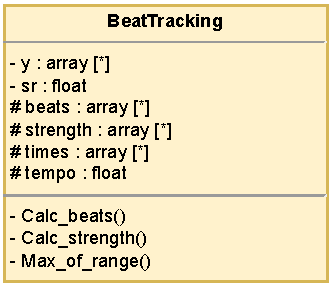
\includegraphics[width = 0.3\linewidth]{obrazky/UML_diagramy_BeatTracking.pdf}
        \caption{Struktura třídy \textit{BeatTracking}}
        \label{fig:BeatTracking_class_diagram}
\end{figure}

Druhá třída s názvem \texttt{ChromaFeatures} je navržena pro získání chroma vlastností dané nahrávky. Obsahuje 4 atributy a 5 metod. Její struktura je zobrazena na diagramu \ref{fig:ChromaFeatures_class_diagram}. Pomocí funkcí jsou vypočteny chroma vektory a paleta barev analyzované skladby. Pro výpočet chroma vlastností jsou používány dvě funkce. První je \texttt{Calc\_chroma\_librosa} využívající algoritmus \texttt{chroma\_cqt} s přídavným předzpracováním signálu a filtrací výsledného pole. Zmíněný výpočet je používán při zvolené náladě \texttt{mood} na hodnoty \uv{happy} a \uv{dancing}. Pro hodnoty \uv{chill} a \uv{hang\_out} je využíváno výpočtu pomocí knihovny madmom ve funkci \texttt{Calc\_chroma\_madmom}. Postup stanovení palety barev, který je naprogramován pomocí funkcí \texttt{Calc\_color\_palete}, \texttt{Generate\_triadic\_colors} a \texttt{Color\_shift} je podrobně popsán v sekci \ref{sec:Color_palete}.

\begin{figure}[H]
    \centering
        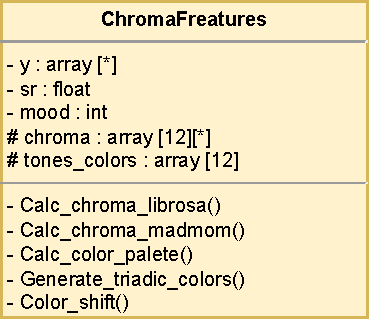
\includegraphics[width = 0.3\linewidth]{obrazky/UML_diagram_ChromaFeatures.pdf}
        \caption{Struktura třídy \textit{ChromaFeatures}}
        \label{fig:ChromaFeatures_class_diagram}
\end{figure}

Pro práci se segmenty je vytvořena třída \textit{Segmentation} a její struktura je zobrazena na obrázku \ref{fig:Segmentation_diagram}. Je využíváno již vypočítaných chroma vektorů, které jsou vstupními parametry funkce z knihovny Librosa. Tato funkce využívá hierarchického aglomerativního shlukování. Pro výpočet je nutné stanovit počet segmentů na které mají být data rozděleny. Počet segmentů je stanoven na základně zvolené nálady. Počty jsou následující: chill -- 8 segmentů, hang out -- 16 segmentů, happy -- 24 segmentů a dancing -- 32 segmentů. Rozdíly jsou vidět na obrázku \ref{fig:Segmentation_segments_comparison}.

\begin{figure}[H]
    \centering
    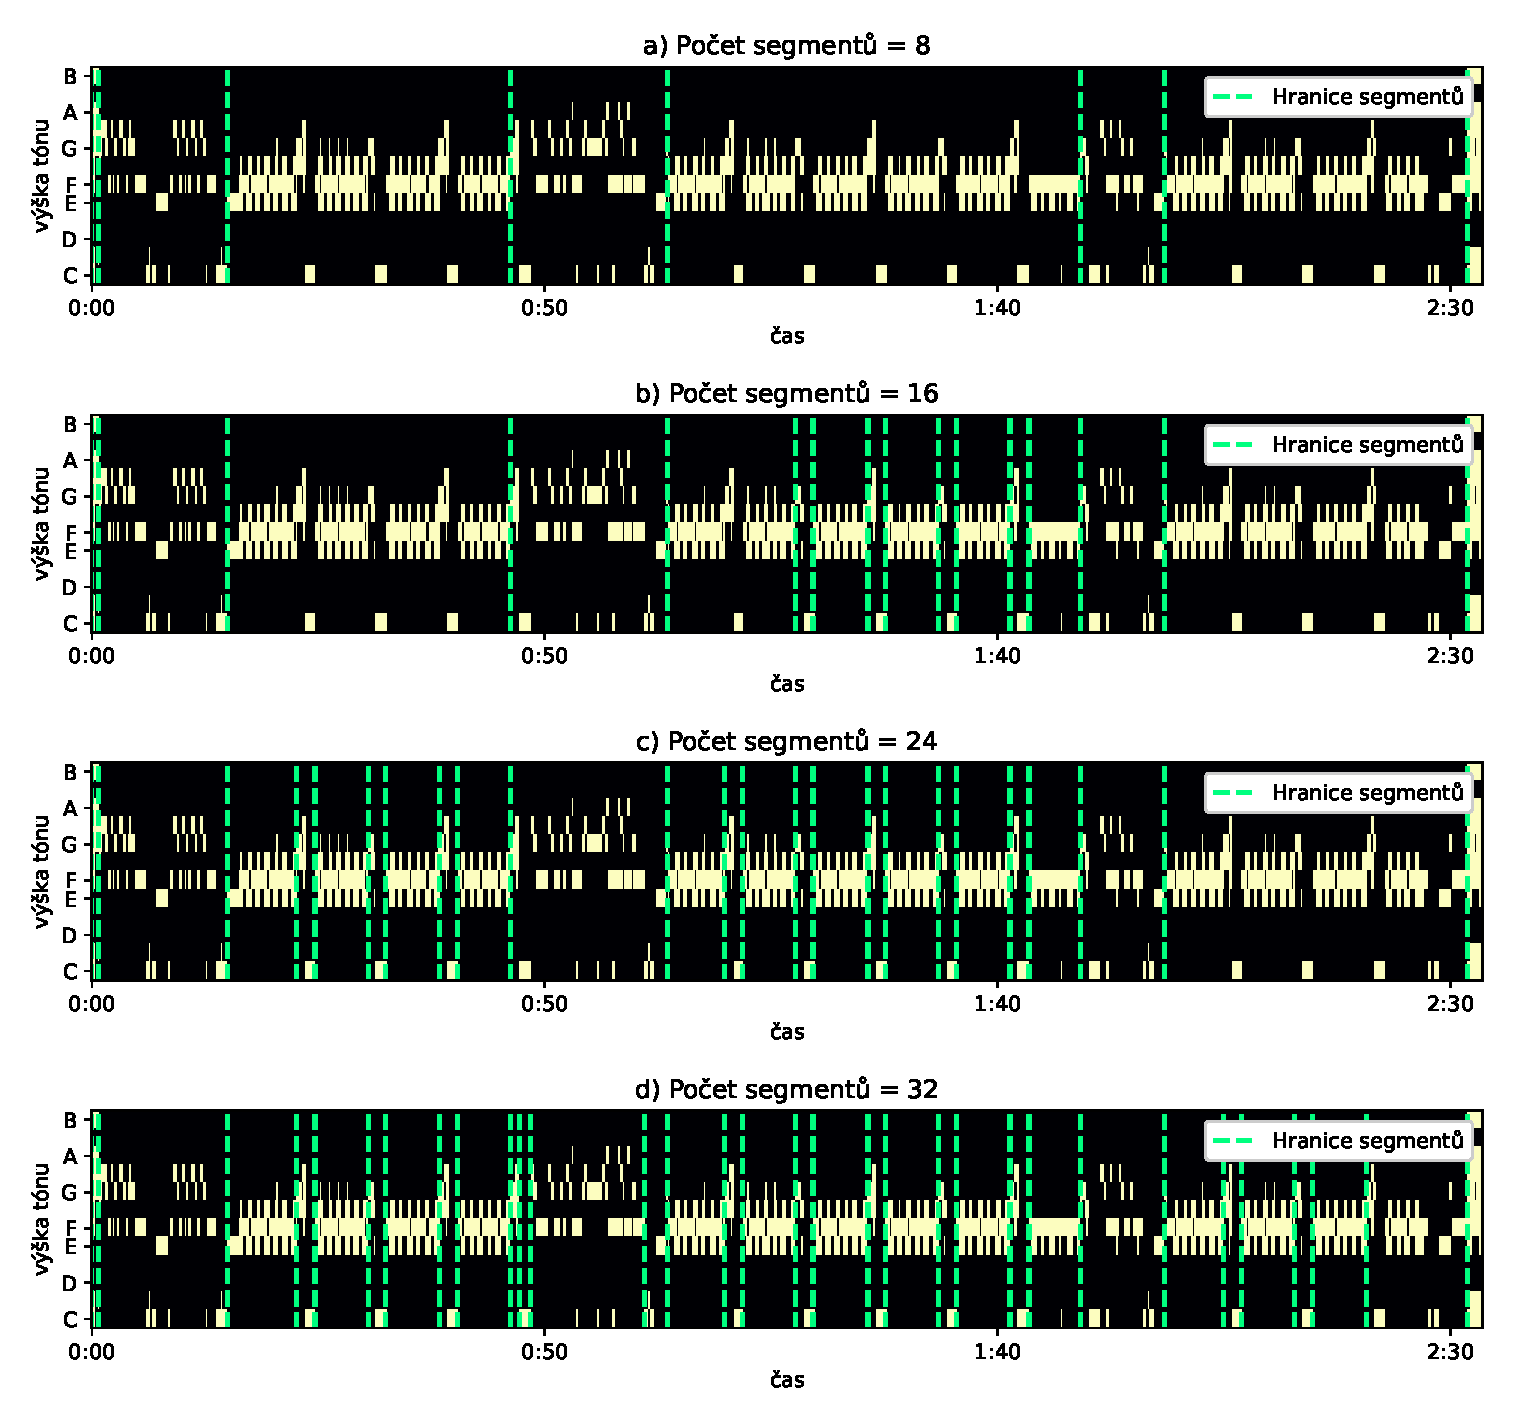
\includegraphics[width = 1\linewidth]{obrazky/Segmentation_segments_comparisons.eps}
    \caption{Porovnání počtu segmentů}
    \label{fig:Segmentation_segments_comparison}
\end{figure}

\begin{figure}[H]
    \centering
    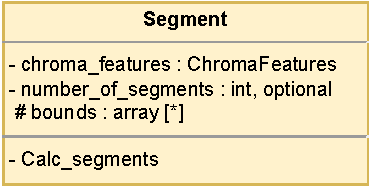
\includegraphics[width = 0.3\linewidth]{obrazky/UML_diagram_Segmentation.pdf}
    \caption{Struktura třídy \texttt{Segment}}
    \label{fig:Segmentation_diagram}
\end{figure}

Metody pro klasifikaci žánrů jsou ve třídě \texttt{GenreClassification}. Ta se skládá ze třech parametrů a třech funkcí. Stanovení žánrů probíhá pomocí naučené neuronové sítě o struktuře čtyřech dvourozměrných konvolučních vrstvách a čtyřech dense vrstev. Mezi konvolučními vrstvami se nachází vždy vrstva dropout a max pooling. Pro její vytvoření je využito balíčků TensorFlow\footnote{TensorFlow je volně šiřitelná knihovna pro strojové učení a umělou inteligenci.} a Keras\footnote{Vysokoúrovňové API rozhraní pro tvorbu neuronových sítí.}. Pro neuronovou síť je nutné aby jí byly předloženy vstupní data vždy o stejné velikosti. Nejprve tedy probíhá předzpracování vstupních dat. K tomu slouží funkce \texttt{Data\_preparation} a \texttt{Calc\_melspec}. V prvním kroku jsou vzorky nahrávky oříznuty na délku 25 s při vzorkovací frekvenci 22050 Hz. Počet vstupních vzorků tedy je $25 * 22050 = 551250$ vzorků. Zkrácená část skladby je následně přepočtena na mel spektrogram s šířkou okna 1024 vzorků. Předzpracovaný signál je nutné převést na tenzory a poté je možné jej vložit do neuronové sítě. Výstupem modelu je tenzor o deseti hodnotách v rozmezí 0-1. Každá hodnota stanovuje pravděpodobnost daného žánru. 

\begin{figure}[H]
    \centering
    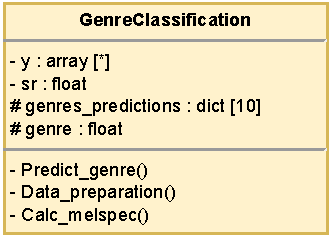
\includegraphics[width = 0.3\linewidth]{obrazky/UML_diagramy_GenreClassification.pdf}
    \caption{Struktura třídy \texttt{GenreClassification}}
    \label{fig:GenreClassification_diagram}
\end{figure}

Model pro klasifikaci žánrů je vytvořen pomocí návodu \uv{Music Classification Using Deep Learning | Python} \cite{Music_classification_using_deep_learning}, který vychází z článku \cite{Music_genre_classification_paper} a teoreticky je popsán v kapitole \ref{sec:Klasifikace_zanru}. 

%TODO: Pokud bude čas přidat postup učení modelu. 

\subsection{Paleta barev} \label{sec:Color_palete}

Paleta barev znázorňuje 12 půltónů s přiřazenými barevnými hodnotami. Barvy jsou stanoveny ve dvou krocích. Jako první jsou určeny 3 základní barvy, které tvoří triadické barevné uspořádání. Celý proces generování probíhá pomocí modelu \acs{HSV}\footnote{HSV -- Hue, Saturation, Value. HSV je barevný model pro uložení informací o barvě pomocí tří hodnot tón, sytost a jas).}. U základní barvy je náhodně vygenerovaná hodnota odstínu v rozmezí 0 až 360. Hodnoty sytosti a jasu jsou přednastavené pro všechny barvy stejně. Ve funkci \texttt{Generate\_ triadic\_colors} jsou vygenerovány zbývající dvě barvy tak, že je hodnota odstínu posunuta vždy o 120 stupňů aby barvy odpovídaly triadickému uspořádání. Aby bylo možné základní barvy přiřadit tónům je nejprve potřeba zjistit, které tři tóny v nahrávce znějí nejčastěji. Matice chroma vektorů je převedena na binární. Hodnoty větší nebo rovny 0,6 jsou zapsány jako 1 hodnoty nižší jsou zapsány jako 0. Následně jsou řádky matice sečteny. Pro každý tón je tedy získána hodnota jak často se vyskytuje ve skladbě. Třem tónům s nejvyšší hodnotou jsou přiřazeny základní barvy. Příklad získaných a přiřazených barev lze vidět na obrázku \ref{fig:Color_palete} a). Zbylé barvy jsou odvozeny od barvy základní pomocí posunutí hodnoty odstínu o $15*i$ stupňů, kde $i$ je počet půltónů od tónu se základní barvou.

\begin{figure}[H]
    \centering
    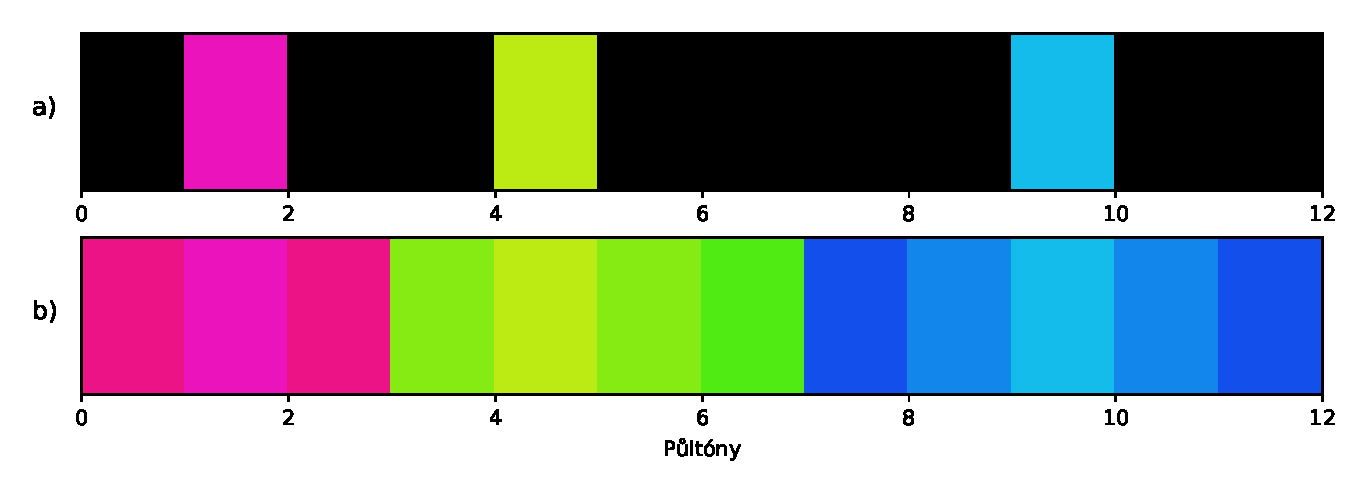
\includegraphics[width = 1\linewidth]{obrazky/Color_palete.eps}
    \caption{Postup generování barevné palety \textbf{a)} Barvy základní, \textbf{b)} Barvy zbylé}
    \label{fig:Color_palete}
\end{figure}

\subsection{Výběr datasetu} \label{sec:Vyber_datasetu}

Blokový diagram výběru datasetu je zobrazen na obrázku \ref{fig:Dataset_selection_diagram}.  Naprogramovaná funkce je pak k nalezení v příloze \ref{code:Dataset_selection}. Funkce má 4 parametry, které jsou důležité pro proces nalezení datasetu. Jedná se o objekt třídy \texttt{GenreClassification}, který poskytuje slovník deseti žánrů s hodnotami pravděpodobnosti pro vloženou skladbu, objekt třídy \texttt{BeatTracking}, sloužící pro zjištění tempa skladby, a hodnotu nálady zvolenou uživatelem. Posledním parametrem je samotná databáze, která představuje list objektů tipu \texttt{Dataset}. Tento list je vždy při spuštění generování načten z přiloženého textového dokumentu, kde je uložen ve formátu \acs{JSON}\footnote{JSON - Je způsob zápisu dat nezávislý na platformě.\cite{JSON}}. Proces se skládá z pěti cyklů. V prvním cyklu jsou procházeny všechny datasety. Pro každý dataset je vnořen další cyklus který postupně projde všechny hodnoty slovníků s žánry a vypočítá rozdíl jejich hodnot s hodnotami získanými z klasifikace žánrů. Tento rozdíl je vždy přičten k celkové hodnotě rozdílu daného datasetu a následně na konec pole \texttt{genres\_difs} obsahujícího hodnoty rozdílů pro zbývající datasety. Po dokončení prvního cyklu pole \texttt{genres\_difs} obsahuje rozdíly v žánrech pro všechny datasety. Následuje druhý cyklus, který v pěti krocích ze zmíněného pole vybere 5 datasetů z nejnižší hodnotou rozdílu žánrů. V posledním cyklu nejprve probíhá kontrola zdali dataset odpovídá zvolené náladě. Pokud podmínku splní je vypočítána hodnota rozdílu tempa mezi doporučeným tempem pro daný dataset a odhadovaným tempem pro vybranou nahrávku. Dataset s nejmenším rozdílem tempa je pak funkcí vrácen jako vybraný dataset pro vložený audio soubor. 

\subsection{Výběr bloku animace} \label{sec:Vyber_bloku_animace}

Řešení vychází ze čtyřech získaných hodnot o audio souboru.

\begin{description}
    \item[Délka audia] je celkovou délku audio souboru vyjádřenou v sekundách. A je vypočítána dle rovnice \ref{rov:Cas_nahravky} kde $N$ je počet vzorků a $f_{vz}$ je vzorkovací frekvence. 

    \begin{equation}
        t_{a} = \frac{N}{f_{vz}}
        \label{rov:Cas_nahravky}
    \end{equation}

    \item[Délka segmentu] -- je vypočítána jako rozdíl času konce segmentu a začátku segmentu. Jednotkou jsou sekundy. 
    \item[Hlasitost audia] -- je vypočítána z knihovny \texttt{Pyloudnorm} popsané v bodě \ref{sec:Pyloudnorm}. Hlasitost je dána v jednotkách LUFS.
    \item[Hlasitost segmentu] -- využívá stejnou funkci jako hlasitost audia akorát jsou do ní vloženy vzorky v rozmezí časů segmentu. 
    \item[Síla počáteční doby] -- udává hodnotu síly nástupu doby a je více popsána v bodě \ref{sec:Parameter_extraction}
    \item[Medián síly dob ve skladbě] -- je stanoven jako medián síly všech dob v nahrávce. 
    \item[Medián síly dob v segmentu] -- je stanoven jako medián  síly všech dob v segmentu. 
\end{description}
Tyto doby jso následně mezi sebou porovnány ve čtyřech blocích. Každý blok se skládá z hodnoty váhy a funkce když. Dva bloky jsou zaměřené na daný segment a určují jak je segment dlouhý a hlasitý v porovnání s celou skladbou. Hodnoty délka a hlasitost skladby jsou před porovnáváním váhovány. Tyto váhy vytváří hranice. Následně jsou mezi sebou hodnoty porovnány pomocí dvou funkcí když. A výsledkem jsou proměnné boolean označující jestli je segment tichý/hlasitý (\texttt{is\_loud}) a dlouhý/krátký (\texttt{is\_long}). Zbylé dva bloky jsou zaměřeny na sílu počáteční doby animace. Tato síla je porovnána z váhovanými hodnotami mediánu síly dob ve skladbě a mediánu síly dob v segmentu. Jejich výstupy označují významnost doby. 

V posledním kroku jsou čtyři získané boolean odpovědi porovnány mezi sebou ve funkci \texttt{Char\_selection}. Logika porovnání je naprogramovaná funkcemi switch a case, v jazyce Python psané jako \texttt{match} a \texttt{case}. První primární blok porovnává proměnné \texttt{is\_long} a \texttt{is\_loud}. Tento blok má 4 možná řešení. V každém řešení je opět vnořena funkce \texttt{match} s dalšími čtyřmi možnými výsledky. Ve vnořeném bloku jsou porovnávány hodnoty významnosti počáteční doby animace \texttt{is\_important\_in\_audio} a \texttt{is\_important\_in\_segment}. Díky takto zvolené struktuře vzniká šestnáct možných řešení. Každé z řešení představuje hodnotu charakteristiky animace na základě které je vybrán blok animace. 

\subsection{Návrhy na zlepšení} \label{sec:Hodnoceni_systemu}

Výsledný program je schopen generovat animace, které do určité míry sedí do zadané skladby. Hodnocení animací je ale velmi individuální akt. Pro navazující práce v oblasti vytvořeného systému by mělo být prioritní vytvoření metod pro hodnocení generovaných algoritmů, aby byl lépe měřitelný vliv úprav algoritmu na výslednou animaci. Níže je popsáno několik oblastí na které by bylo zajímavé upnout budoucí výzkum a mohlo by tak dojít ke zlepšení vizuální stránky generovaných animací. 
\begin{itemize}
    \item Získání lepších informací o jednotlivých dobách. Například analýza silných dob a slabých dob. V angličtině používané názvy \uv{downbeat} a \uv{upbeat}. Tyto informace by umožnili mnohem lepší kontrolu nad přiřazováním začátků a konců bloků tak aby lépe zapadaly do rytmické struktury skladby.
    \item Segmentace nahrávky by mohla obsahovat více informací o daném segmentu. Parametry jako role segmentu ve skladbě, počet taktů v segmentu by mohly pozitivně ovlivnit výběr vhodného bloku animace.
    \item Testování odlišných hodnot vah a následné zaznamenávání vlivu změn vah na vizuální změny animace. Stejně tak nastavení rozhodovací logické struktury při výběru bloků animací. Díky tomu je možné získat lepší přehled o vlivu jednotlivých parametrů na výslednou animaci. To následně umožňuje vytvořit nastavení pro různé nálady, žánry či tempa skladby. 
    \item Aplikace momentálně pracuje s umisťováním jednotlivých bloků animací za sebe. Systém Spectoda však umožňuje aby se v jednu chvíli překrývalo až šestnáct animací. Proto jako další krok pro vylepšení může být zaměření právě na překrývání a prolívání animací mezi sebou. 
    \item V neposlední řadě je rychlost generování. V případě komerčního užití by bylo žádoucí proces generování zefektivnit aby uživatel nemusel čekat na vygenerovanou animaci několik desítek sekund. 
\end{itemize}

